\documentclass[twoside]{book}

% Packages required by doxygen
\usepackage{fixltx2e}
\usepackage{calc}
\usepackage{doxygen}
\usepackage[export]{adjustbox} % also loads graphicx
\usepackage{graphicx}
\usepackage[utf8]{inputenc}
\usepackage{makeidx}
\usepackage{multicol}
\usepackage{multirow}
\PassOptionsToPackage{warn}{textcomp}
\usepackage{textcomp}
\usepackage[nointegrals]{wasysym}
\usepackage[table]{xcolor}

% Font selection
\usepackage[T1]{fontenc}
\usepackage[scaled=.90]{helvet}
\usepackage{courier}
\usepackage{amssymb}
\usepackage{sectsty}
\renewcommand{\familydefault}{\sfdefault}
\allsectionsfont{%
  \fontseries{bc}\selectfont%
  \color{darkgray}%
}
\renewcommand{\DoxyLabelFont}{%
  \fontseries{bc}\selectfont%
  \color{darkgray}%
}
\newcommand{\+}{\discretionary{\mbox{\scriptsize$\hookleftarrow$}}{}{}}

% Page & text layout
\usepackage{geometry}
\geometry{%
  a4paper,%
  top=2.5cm,%
  bottom=2.5cm,%
  left=2.5cm,%
  right=2.5cm%
}
\tolerance=750
\hfuzz=15pt
\hbadness=750
\setlength{\emergencystretch}{15pt}
\setlength{\parindent}{0cm}
\setlength{\parskip}{3ex plus 2ex minus 2ex}
\makeatletter
\renewcommand{\paragraph}{%
  \@startsection{paragraph}{4}{0ex}{-1.0ex}{1.0ex}{%
    \normalfont\normalsize\bfseries\SS@parafont%
  }%
}
\renewcommand{\subparagraph}{%
  \@startsection{subparagraph}{5}{0ex}{-1.0ex}{1.0ex}{%
    \normalfont\normalsize\bfseries\SS@subparafont%
  }%
}
\makeatother

% Headers & footers
\usepackage{fancyhdr}
\pagestyle{fancyplain}
\fancyhead[LE]{\fancyplain{}{\bfseries\thepage}}
\fancyhead[CE]{\fancyplain{}{}}
\fancyhead[RE]{\fancyplain{}{\bfseries\leftmark}}
\fancyhead[LO]{\fancyplain{}{\bfseries\rightmark}}
\fancyhead[CO]{\fancyplain{}{}}
\fancyhead[RO]{\fancyplain{}{\bfseries\thepage}}
\fancyfoot[LE]{\fancyplain{}{}}
\fancyfoot[CE]{\fancyplain{}{}}
\fancyfoot[RE]{\fancyplain{}{\bfseries\scriptsize Generated by Doxygen }}
\fancyfoot[LO]{\fancyplain{}{\bfseries\scriptsize Generated by Doxygen }}
\fancyfoot[CO]{\fancyplain{}{}}
\fancyfoot[RO]{\fancyplain{}{}}
\renewcommand{\footrulewidth}{0.4pt}
\renewcommand{\chaptermark}[1]{%
  \markboth{#1}{}%
}
\renewcommand{\sectionmark}[1]{%
  \markright{\thesection\ #1}%
}

% Indices & bibliography
\usepackage{natbib}
\usepackage[titles]{tocloft}
\setcounter{tocdepth}{3}
\setcounter{secnumdepth}{5}
\makeindex

% Hyperlinks (required, but should be loaded last)
\usepackage{ifpdf}
\ifpdf
  \usepackage[pdftex,pagebackref=true]{hyperref}
\else
  \usepackage[ps2pdf,pagebackref=true]{hyperref}
\fi
\hypersetup{%
  colorlinks=true,%
  linkcolor=blue,%
  citecolor=blue,%
  unicode%
}

% Custom commands
\newcommand{\clearemptydoublepage}{%
  \newpage{\pagestyle{empty}\cleardoublepage}%
}

\usepackage{caption}
\captionsetup{labelsep=space,justification=centering,font={bf},singlelinecheck=off,skip=4pt,position=top}

%===== C O N T E N T S =====

\begin{document}

% Titlepage & ToC
\hypersetup{pageanchor=false,
             bookmarksnumbered=true,
             pdfencoding=unicode
            }
\pagenumbering{alph}
\begin{titlepage}
\vspace*{7cm}
\begin{center}%
{\Large Polygon-\/\+Triangulate \\[1ex]\large 1.\+0 }\\
\vspace*{1cm}
{\large Generated by Doxygen 1.8.13}\\
\end{center}
\end{titlepage}
\clearemptydoublepage
\pagenumbering{roman}
\tableofcontents
\clearemptydoublepage
\pagenumbering{arabic}
\hypersetup{pageanchor=true}

%--- Begin generated contents ---
\chapter{D\+C\+E\+L-\/\+Polygon-\/\+Triangulate}
\label{index}\hypertarget{index}{}C++ Implementation polygon triangulation algorithm making use of \hyperlink{structDCEL}{D\+C\+EL}; Time Complexity O(nlogn); Done as part of the Computational Geometry Course at B\+I\+TS Pilani -\/ Hyderabad, under Prof. Tathagata Ray.

\subsection*{Instructions}

{\ttfamily cd src}

{\ttfamily make clean}

{\ttfamily make}

{\ttfamily ./triangulate}

\subsection*{T\+O-\/\+DO\+:}


\begin{DoxyItemize}
\item \mbox{[}X\mbox{]} \hyperlink{structDCEL}{D\+C\+EL}
\item \mbox{[}X\mbox{]} Make Monotone
\item \mbox{[}X\mbox{]} Triangulate
\item \mbox{[}X\mbox{]} Performance Analysis
\item \mbox{[}X\mbox{]} Stress test with large cases (Important)
\item \mbox{[}X\mbox{]} Documentation, Comments, A\+PI Interface, Directory Structure
\end{DoxyItemize}

\subsection*{Support}

Contact Harivallabha Rangarajan or Sathyaram, for any questions regarding running the code.

\subsection*{Authors}


\begin{DoxyItemize}
\item Sathyaram, Department of Chemistry and Computer Science, B\+I\+TS Pilani -\/ Hyderabad.
\item Harivallabha Rangarajan, Department of Mathematics and Computer Science, B\+I\+TS Pilani-\/\+Hyderabad.
\end{DoxyItemize}

\subsection*{Acknowledgements}

We acknowledge Geogebra, and Desmos for helping us visualize. Thank you! 
\chapter{Class Index}
\section{Class List}
Here are the classes, structs, unions and interfaces with brief descriptions\+:\begin{DoxyCompactList}
\item\contentsline{section}{\hyperlink{structDCEL}{D\+C\+EL} \\*\hyperlink{structDCEL}{D\+C\+EL} struct\+: The main \hyperlink{structDCEL}{D\+C\+EL} data structure that is used to represent the regions. Implements handling for different kinds of vertices through its member functions; Also implements the make-\/montone function that decomposes the polygon into monotone subcomponents }{\pageref{structDCEL}}{}
\item\contentsline{section}{\hyperlink{structEdge}{Edge} \\*\hyperlink{structEdge}{Edge} struct\+: has \hyperlink{structEdge}{Edge} data members that store pointers to twin, next and prev has \hyperlink{structVertex}{Vertex} data members that store pointers to origin and helper has a \hyperlink{structFace}{Face} data member that points to the incident face }{\pageref{structEdge}}{}
\item\contentsline{section}{\hyperlink{structDCEL_1_1EdgePtrComp}{D\+C\+E\+L\+::\+Edge\+Ptr\+Comp} \\*\hyperlink{structDCEL_1_1EdgePtrComp}{Edge\+Ptr\+Comp} Struct\+: Helper struct to compare two edges using the Tau structure }{\pageref{structDCEL_1_1EdgePtrComp}}{}
\item\contentsline{section}{\hyperlink{structFace}{Face} \\*\hyperlink{structFace}{Face} struct\+: Contains a pointer to the corresponding \hyperlink{structEdge}{Edge} }{\pageref{structFace}}{}
\item\contentsline{section}{\hyperlink{structVertex}{Vertex} \\*\hyperlink{structVertex}{Vertex} struct\+: has a data member type that identifies the vertex type among start, end, regular, split, merge has two data members x and y corresponding to the x and y co-\/ordinates of the vertex respectively overloads comparison operator }{\pageref{structVertex}}{}
\item\contentsline{section}{\hyperlink{structDCEL_1_1VertexPtrComp}{D\+C\+E\+L\+::\+Vertex\+Ptr\+Comp} \\*\hyperlink{structDCEL_1_1VertexPtrComp}{Vertex\+Ptr\+Comp} Struct\+: Helper struct to compare two vertex pointers }{\pageref{structDCEL_1_1VertexPtrComp}}{}
\end{DoxyCompactList}

\chapter{File Index}
\section{File List}
Here is a list of all documented files with brief descriptions\+:\begin{DoxyCompactList}
\item\contentsline{section}{src/\hyperlink{data__structure_8hpp}{data\+\_\+structure.\+hpp} }{\pageref{data__structure_8hpp}}{}
\item\contentsline{section}{src/\hyperlink{main_8cpp}{main.\+cpp} }{\pageref{main_8cpp}}{}
\item\contentsline{section}{src/\hyperlink{utils_8hpp}{utils.\+hpp} }{\pageref{utils_8hpp}}{}
\end{DoxyCompactList}

\chapter{Class Documentation}
\hypertarget{structDCEL}{}\section{D\+C\+EL Struct Reference}
\label{structDCEL}\index{D\+C\+EL@{D\+C\+EL}}


\hyperlink{structDCEL}{D\+C\+EL} struct\+: The main \hyperlink{structDCEL}{D\+C\+EL} data structure that is used to represent the regions. Implements handling for different kinds of vertices through its member functions; Also implements the make-\/montone function that decomposes the polygon into monotone subcomponents.  




{\ttfamily \#include $<$data\+\_\+structure.\+hpp$>$}

\subsection*{Classes}
\begin{DoxyCompactItemize}
\item 
struct \hyperlink{structDCEL_1_1EdgePtrComp}{Edge\+Ptr\+Comp}
\begin{DoxyCompactList}\small\item\em \hyperlink{structDCEL_1_1EdgePtrComp}{Edge\+Ptr\+Comp} Struct\+: Helper struct to compare two edges using the Tau structure. \end{DoxyCompactList}\item 
struct \hyperlink{structDCEL_1_1VertexPtrComp}{Vertex\+Ptr\+Comp}
\begin{DoxyCompactList}\small\item\em \hyperlink{structDCEL_1_1VertexPtrComp}{Vertex\+Ptr\+Comp} Struct\+: Helper struct to compare two vertex pointers. \end{DoxyCompactList}\end{DoxyCompactItemize}
\subsection*{Public Member Functions}
\begin{DoxyCompactItemize}
\item 
\mbox{\Hypertarget{structDCEL_a9ba659c772047cd7867f49945a557152}\label{structDCEL_a9ba659c772047cd7867f49945a557152}} 
virtual \hyperlink{structEdge}{Edge} $\ast$ {\bfseries get\+\_\+support} (\hyperlink{structVertex}{Vertex} $\ast$v, set$<$ \hyperlink{structEdge}{Edge} $\ast$, \hyperlink{structDCEL_1_1EdgePtrComp}{Edge\+Ptr\+Comp} $>$ \&Tau)
\item 
\mbox{\Hypertarget{structDCEL_a9efcd9a2e78efac4f71931946cdff606}\label{structDCEL_a9efcd9a2e78efac4f71931946cdff606}} 
virtual void {\bfseries handle\+\_\+start} (\hyperlink{structVertex}{Vertex} $\ast$v, set$<$ \hyperlink{structEdge}{Edge} $\ast$, \hyperlink{structDCEL_1_1EdgePtrComp}{Edge\+Ptr\+Comp} $>$ \&Tau)
\item 
\mbox{\Hypertarget{structDCEL_a8fd85fb5dbe52c27fd49e465222ea05d}\label{structDCEL_a8fd85fb5dbe52c27fd49e465222ea05d}} 
virtual void {\bfseries handle\+\_\+end} (\hyperlink{structVertex}{Vertex} $\ast$v, set$<$ \hyperlink{structEdge}{Edge} $\ast$, \hyperlink{structDCEL_1_1EdgePtrComp}{Edge\+Ptr\+Comp} $>$ \&Tau)
\item 
\mbox{\Hypertarget{structDCEL_afd1b47312ef100985cb59f5019f49e01}\label{structDCEL_afd1b47312ef100985cb59f5019f49e01}} 
virtual void {\bfseries add\+\_\+diagnol} (\hyperlink{structVertex}{Vertex} $\ast$helper, \hyperlink{structVertex}{Vertex} $\ast$v)
\item 
\mbox{\Hypertarget{structDCEL_a1cfc774b59a157b111be2db2ad6a2f5d}\label{structDCEL_a1cfc774b59a157b111be2db2ad6a2f5d}} 
virtual void {\bfseries handle\+\_\+split} (\hyperlink{structVertex}{Vertex} $\ast$v, set$<$ \hyperlink{structEdge}{Edge} $\ast$, \hyperlink{structDCEL_1_1EdgePtrComp}{Edge\+Ptr\+Comp} $>$ \&Tau)
\item 
\mbox{\Hypertarget{structDCEL_a4567bbbac7a706cf4d51199e63e7ac5b}\label{structDCEL_a4567bbbac7a706cf4d51199e63e7ac5b}} 
virtual void {\bfseries handle\+\_\+merge} (\hyperlink{structVertex}{Vertex} $\ast$v, set$<$ \hyperlink{structEdge}{Edge} $\ast$, \hyperlink{structDCEL_1_1EdgePtrComp}{Edge\+Ptr\+Comp} $>$ \&Tau)
\item 
\mbox{\Hypertarget{structDCEL_a0e9b658feb6fadea3ca47bd91eca85bc}\label{structDCEL_a0e9b658feb6fadea3ca47bd91eca85bc}} 
virtual void {\bfseries handle\+\_\+regular} (\hyperlink{structVertex}{Vertex} $\ast$v, set$<$ \hyperlink{structEdge}{Edge} $\ast$, \hyperlink{structDCEL_1_1EdgePtrComp}{Edge\+Ptr\+Comp} $>$ \&Tau)
\item 
\mbox{\Hypertarget{structDCEL_a5713f17e9d21cc2a77f49bd8dbf0821d}\label{structDCEL_a5713f17e9d21cc2a77f49bd8dbf0821d}} 
virtual void {\bfseries make\+\_\+monotone} ()
\end{DoxyCompactItemize}
\subsection*{Public Attributes}
\begin{DoxyCompactItemize}
\item 
\mbox{\Hypertarget{structDCEL_ad95be5ea47a3e065ac3db8077ed8b11f}\label{structDCEL_ad95be5ea47a3e065ac3db8077ed8b11f}} 
int {\bfseries n}
\item 
\mbox{\Hypertarget{structDCEL_ade0e662c344e8b99fd3276c1694439f3}\label{structDCEL_ade0e662c344e8b99fd3276c1694439f3}} 
vector$<$ \hyperlink{structVertex}{Vertex} $\ast$ $>$ {\bfseries vertices}
\item 
\mbox{\Hypertarget{structDCEL_a2c071fc3e862f820c53610c8618aa461}\label{structDCEL_a2c071fc3e862f820c53610c8618aa461}} 
vector$<$ \hyperlink{structEdge}{Edge} $\ast$ $>$ {\bfseries edges}
\item 
\mbox{\Hypertarget{structDCEL_a2d7fd9417422b18f18e8c55f1d1f49e2}\label{structDCEL_a2d7fd9417422b18f18e8c55f1d1f49e2}} 
vector$<$ \hyperlink{structFace}{Face} $\ast$ $>$ {\bfseries faces}
\item 
\mbox{\Hypertarget{structDCEL_ad92c73a3c5980d727f9ec9f068bc2b0e}\label{structDCEL_ad92c73a3c5980d727f9ec9f068bc2b0e}} 
vector$<$ \hyperlink{structFace}{Face} $\ast$ $>$ {\bfseries ymonotones}
\item 
\mbox{\Hypertarget{structDCEL_aa88d0e054d12b2444fa45aa2da22d988}\label{structDCEL_aa88d0e054d12b2444fa45aa2da22d988}} 
int {\bfseries monotone\+\_\+edges}
\end{DoxyCompactItemize}


\subsection{Detailed Description}
\hyperlink{structDCEL}{D\+C\+EL} struct\+: The main \hyperlink{structDCEL}{D\+C\+EL} data structure that is used to represent the regions. Implements handling for different kinds of vertices through its member functions; Also implements the make-\/montone function that decomposes the polygon into monotone subcomponents. 

The documentation for this struct was generated from the following files\+:\begin{DoxyCompactItemize}
\item 
src/\hyperlink{data__structure_8hpp}{data\+\_\+structure.\+hpp}\item 
src/data\+\_\+structure.\+cpp\end{DoxyCompactItemize}

\hypertarget{structEdge}{}\section{Edge Struct Reference}
\label{structEdge}\index{Edge@{Edge}}


\hyperlink{structEdge}{Edge} struct\+: has \hyperlink{structEdge}{Edge} data members that store pointers to twin, next and prev has \hyperlink{structVertex}{Vertex} data members that store pointers to origin and helper has a \hyperlink{structFace}{Face} data member that points to the incident face.  




{\ttfamily \#include $<$data\+\_\+structure.\+hpp$>$}



Collaboration diagram for Edge\+:
\nopagebreak
\begin{figure}[H]
\begin{center}
\leavevmode
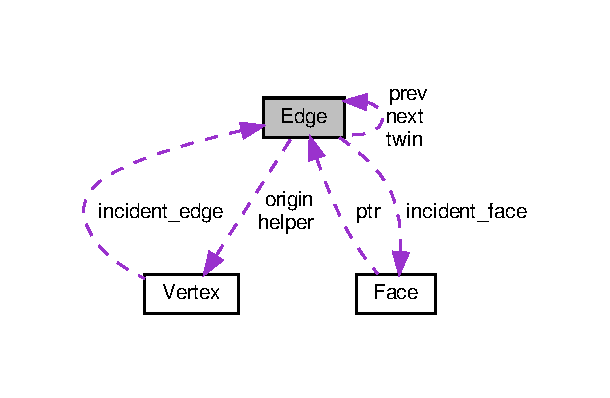
\includegraphics[width=293pt]{structEdge__coll__graph}
\end{center}
\end{figure}
\subsection*{Public Member Functions}
\begin{DoxyCompactItemize}
\item 
\hyperlink{structVertex}{Vertex} $\ast$ \hyperlink{structEdge_a3fe7e84f2ef319dbe30d48c4d268832d}{get\+\_\+helper} ()
\item 
\mbox{\Hypertarget{structEdge_a8570e2155927300a0769e90a284d554c}\label{structEdge_a8570e2155927300a0769e90a284d554c}} 
void {\bfseries set\+\_\+helper} (\hyperlink{structVertex}{Vertex} $\ast$v)
\item 
\mbox{\Hypertarget{structEdge_a497ea9939f608695dde42a4362ff4714}\label{structEdge_a497ea9939f608695dde42a4362ff4714}} 
bool {\bfseries operator$<$} (const \hyperlink{structEdge}{Edge} \&rhs)
\end{DoxyCompactItemize}
\subsection*{Public Attributes}
\begin{DoxyCompactItemize}
\item 
\mbox{\Hypertarget{structEdge_a45fb96b9c533f450b1f7f4a03a353d96}\label{structEdge_a45fb96b9c533f450b1f7f4a03a353d96}} 
struct \hyperlink{structEdge}{Edge} $\ast$ {\bfseries twin}
\item 
\mbox{\Hypertarget{structEdge_a3cf3d57ae65110456b5d809a658757fc}\label{structEdge_a3cf3d57ae65110456b5d809a658757fc}} 
struct \hyperlink{structEdge}{Edge} $\ast$ {\bfseries next}
\item 
\mbox{\Hypertarget{structEdge_ae4477dab61b692f0a1bc3241e3bfaddd}\label{structEdge_ae4477dab61b692f0a1bc3241e3bfaddd}} 
struct \hyperlink{structEdge}{Edge} $\ast$ {\bfseries prev}
\item 
\mbox{\Hypertarget{structEdge_a2de3c697d4a77673df6bcac7cc7b5b08}\label{structEdge_a2de3c697d4a77673df6bcac7cc7b5b08}} 
struct \hyperlink{structVertex}{Vertex} $\ast$ {\bfseries origin}
\item 
\mbox{\Hypertarget{structEdge_abb06ddf30396af97c26a5a43bec10ef7}\label{structEdge_abb06ddf30396af97c26a5a43bec10ef7}} 
struct \hyperlink{structVertex}{Vertex} $\ast$ {\bfseries helper}
\item 
\mbox{\Hypertarget{structEdge_aeca88bcc64d0e3a1393f87613bfc5fe8}\label{structEdge_aeca88bcc64d0e3a1393f87613bfc5fe8}} 
struct \hyperlink{structFace}{Face} $\ast$ {\bfseries incident\+\_\+face}
\end{DoxyCompactItemize}


\subsection{Detailed Description}
\hyperlink{structEdge}{Edge} struct\+: has \hyperlink{structEdge}{Edge} data members that store pointers to twin, next and prev has \hyperlink{structVertex}{Vertex} data members that store pointers to origin and helper has a \hyperlink{structFace}{Face} data member that points to the incident face. 

\subsection{Member Function Documentation}
\mbox{\Hypertarget{structEdge_a3fe7e84f2ef319dbe30d48c4d268832d}\label{structEdge_a3fe7e84f2ef319dbe30d48c4d268832d}} 
\index{Edge@{Edge}!get\+\_\+helper@{get\+\_\+helper}}
\index{get\+\_\+helper@{get\+\_\+helper}!Edge@{Edge}}
\subsubsection{\texorpdfstring{get\+\_\+helper()}{get\_helper()}}
{\footnotesize\ttfamily \hyperlink{structVertex}{Vertex}$\ast$ Edge\+::get\+\_\+helper (\begin{DoxyParamCaption}{ }\end{DoxyParamCaption})\hspace{0.3cm}{\ttfamily [inline]}}

Function that returns the helper vertex 

The documentation for this struct was generated from the following file\+:\begin{DoxyCompactItemize}
\item 
src/\hyperlink{data__structure_8hpp}{data\+\_\+structure.\+hpp}\end{DoxyCompactItemize}

\hypertarget{structDCEL_1_1EdgePtrComp}{}\section{D\+C\+EL\+:\+:Edge\+Ptr\+Comp Struct Reference}
\label{structDCEL_1_1EdgePtrComp}\index{D\+C\+E\+L\+::\+Edge\+Ptr\+Comp@{D\+C\+E\+L\+::\+Edge\+Ptr\+Comp}}


\hyperlink{structDCEL_1_1EdgePtrComp}{Edge\+Ptr\+Comp} Struct\+: Helper struct to compare two edges using the Tau structure.  




{\ttfamily \#include $<$data\+\_\+structure.\+hpp$>$}

\subsection*{Public Member Functions}
\begin{DoxyCompactItemize}
\item 
\mbox{\Hypertarget{structDCEL_1_1EdgePtrComp_adeed54ffca3d038aa5c2612455662c40}\label{structDCEL_1_1EdgePtrComp_adeed54ffca3d038aa5c2612455662c40}} 
bool {\bfseries operator()} (const \hyperlink{structEdge}{Edge} $\ast$lhs, const \hyperlink{structEdge}{Edge} $\ast$rhs) const
\end{DoxyCompactItemize}


\subsection{Detailed Description}
\hyperlink{structDCEL_1_1EdgePtrComp}{Edge\+Ptr\+Comp} Struct\+: Helper struct to compare two edges using the Tau structure. 

The documentation for this struct was generated from the following file\+:\begin{DoxyCompactItemize}
\item 
src/\hyperlink{data__structure_8hpp}{data\+\_\+structure.\+hpp}\end{DoxyCompactItemize}

\hypertarget{structFace}{}\section{Face Struct Reference}
\label{structFace}\index{Face@{Face}}


\hyperlink{structFace}{Face} struct\+: Contains a pointer to the corresponding \hyperlink{structEdge}{Edge}.  




{\ttfamily \#include $<$data\+\_\+structure.\+hpp$>$}



Collaboration diagram for Face\+:
\nopagebreak
\begin{figure}[H]
\begin{center}
\leavevmode
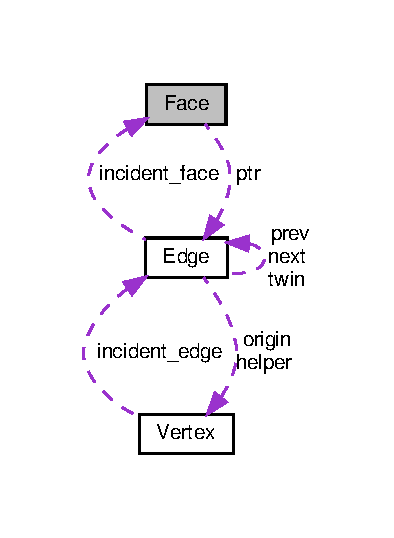
\includegraphics[width=189pt]{structFace__coll__graph}
\end{center}
\end{figure}
\subsection*{Public Attributes}
\begin{DoxyCompactItemize}
\item 
\mbox{\Hypertarget{structFace_a21890b9e9ec72f7f79abf7ef5592d5fd}\label{structFace_a21890b9e9ec72f7f79abf7ef5592d5fd}} 
struct \hyperlink{structEdge}{Edge} $\ast$ {\bfseries ptr}
\end{DoxyCompactItemize}


\subsection{Detailed Description}
\hyperlink{structFace}{Face} struct\+: Contains a pointer to the corresponding \hyperlink{structEdge}{Edge}. 

The documentation for this struct was generated from the following file\+:\begin{DoxyCompactItemize}
\item 
src/\hyperlink{data__structure_8hpp}{data\+\_\+structure.\+hpp}\end{DoxyCompactItemize}

\hypertarget{structVertex}{}\section{Vertex Struct Reference}
\label{structVertex}\index{Vertex@{Vertex}}


\hyperlink{structVertex}{Vertex} struct\+: has a data member type that identifies the vertex type among start, end, regular, split, merge has two data members x and y corresponding to the x and y co-\/ordinates of the vertex respectively overloads comparison operator.  




{\ttfamily \#include $<$data\+\_\+structure.\+hpp$>$}



Collaboration diagram for Vertex\+:
\nopagebreak
\begin{figure}[H]
\begin{center}
\leavevmode
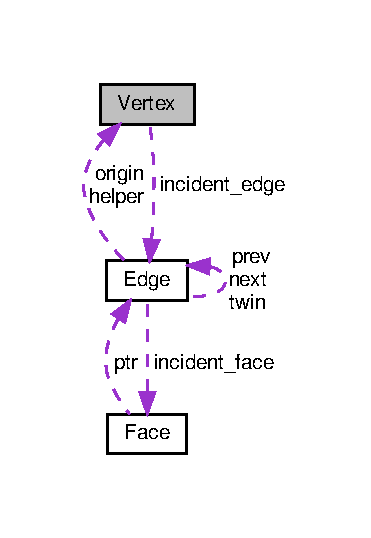
\includegraphics[width=178pt]{structVertex__coll__graph}
\end{center}
\end{figure}
\subsection*{Public Member Functions}
\begin{DoxyCompactItemize}
\item 
\hyperlink{structVertex_a2927de87e482ddebbb18abf7f811c6c3}{Vertex} (double x, double y)
\item 
\mbox{\Hypertarget{structVertex_a666b9e590347fa9a3e10d468ae6d6836}\label{structVertex_a666b9e590347fa9a3e10d468ae6d6836}} 
bool {\bfseries operator$<$} (const \hyperlink{structVertex}{Vertex} \&rhs)
\end{DoxyCompactItemize}
\subsection*{Public Attributes}
\begin{DoxyCompactItemize}
\item 
\mbox{\Hypertarget{structVertex_a9bbbbd39330811b13f4a5de0583b84ea}\label{structVertex_a9bbbbd39330811b13f4a5de0583b84ea}} 
int {\bfseries type}
\item 
\mbox{\Hypertarget{structVertex_af2602132c3297d81bc9f8ee54867445b}\label{structVertex_af2602132c3297d81bc9f8ee54867445b}} 
double {\bfseries x}
\item 
\mbox{\Hypertarget{structVertex_a7563c83da86f4a0831144bc823fec2b0}\label{structVertex_a7563c83da86f4a0831144bc823fec2b0}} 
double {\bfseries y}
\item 
\mbox{\Hypertarget{structVertex_a668b3aa9231e5aab5799aca4ada528db}\label{structVertex_a668b3aa9231e5aab5799aca4ada528db}} 
struct \hyperlink{structEdge}{Edge} $\ast$ {\bfseries incident\+\_\+edge}
\end{DoxyCompactItemize}


\subsection{Detailed Description}
\hyperlink{structVertex}{Vertex} struct\+: has a data member type that identifies the vertex type among start, end, regular, split, merge has two data members x and y corresponding to the x and y co-\/ordinates of the vertex respectively overloads comparison operator. 

\subsection{Constructor \& Destructor Documentation}
\mbox{\Hypertarget{structVertex_a2927de87e482ddebbb18abf7f811c6c3}\label{structVertex_a2927de87e482ddebbb18abf7f811c6c3}} 
\index{Vertex@{Vertex}!Vertex@{Vertex}}
\index{Vertex@{Vertex}!Vertex@{Vertex}}
\subsubsection{\texorpdfstring{Vertex()}{Vertex()}}
{\footnotesize\ttfamily Vertex\+::\+Vertex (\begin{DoxyParamCaption}\item[{double}]{x,  }\item[{double}]{y }\end{DoxyParamCaption})\hspace{0.3cm}{\ttfamily [inline]}}

Constructor to initialize the co-\/ordinates of the vertex 

The documentation for this struct was generated from the following file\+:\begin{DoxyCompactItemize}
\item 
src/\hyperlink{data__structure_8hpp}{data\+\_\+structure.\+hpp}\end{DoxyCompactItemize}

\hypertarget{structDCEL_1_1VertexPtrComp}{}\section{D\+C\+EL\+:\+:Vertex\+Ptr\+Comp Struct Reference}
\label{structDCEL_1_1VertexPtrComp}\index{D\+C\+E\+L\+::\+Vertex\+Ptr\+Comp@{D\+C\+E\+L\+::\+Vertex\+Ptr\+Comp}}


\hyperlink{structDCEL_1_1VertexPtrComp}{Vertex\+Ptr\+Comp} Struct\+: Helper struct to compare two vertex pointers.  




{\ttfamily \#include $<$data\+\_\+structure.\+hpp$>$}

\subsection*{Public Member Functions}
\begin{DoxyCompactItemize}
\item 
\mbox{\Hypertarget{structDCEL_1_1VertexPtrComp_a6058135de8dda7cf6a998939e21c415e}\label{structDCEL_1_1VertexPtrComp_a6058135de8dda7cf6a998939e21c415e}} 
bool {\bfseries operator()} (const \hyperlink{structVertex}{Vertex} $\ast$lhs, const \hyperlink{structVertex}{Vertex} $\ast$rhs) const
\end{DoxyCompactItemize}


\subsection{Detailed Description}
\hyperlink{structDCEL_1_1VertexPtrComp}{Vertex\+Ptr\+Comp} Struct\+: Helper struct to compare two vertex pointers. 

The documentation for this struct was generated from the following file\+:\begin{DoxyCompactItemize}
\item 
src/\hyperlink{data__structure_8hpp}{data\+\_\+structure.\+hpp}\end{DoxyCompactItemize}

\chapter{File Documentation}
\hypertarget{data__structure_8hpp}{}\section{src/data\+\_\+structure.hpp File Reference}
\label{data__structure_8hpp}\index{src/data\+\_\+structure.\+hpp@{src/data\+\_\+structure.\+hpp}}
{\ttfamily \#include \char`\"{}utils.\+hpp\char`\"{}}\newline
Include dependency graph for data\+\_\+structure.\+hpp\+:\nopagebreak
\begin{figure}[H]
\begin{center}
\leavevmode
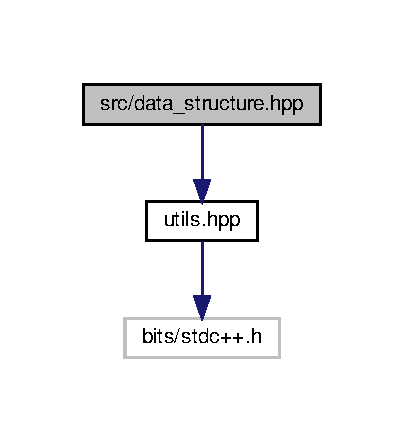
\includegraphics[width=194pt]{data__structure_8hpp__incl}
\end{center}
\end{figure}
This graph shows which files directly or indirectly include this file\+:\nopagebreak
\begin{figure}[H]
\begin{center}
\leavevmode
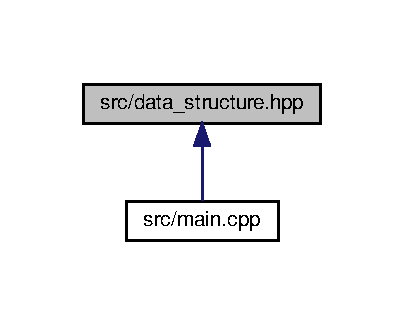
\includegraphics[width=194pt]{data__structure_8hpp__dep__incl}
\end{center}
\end{figure}
\subsection*{Classes}
\begin{DoxyCompactItemize}
\item 
struct \hyperlink{structVertex}{Vertex}
\begin{DoxyCompactList}\small\item\em \hyperlink{structVertex}{Vertex} struct\+: has a data member type that identifies the vertex type among start, end, regular, split, merge has two data members x and y corresponding to the x and y co-\/ordinates of the vertex respectively overloads comparison operator. \end{DoxyCompactList}\item 
struct \hyperlink{structEdge}{Edge}
\begin{DoxyCompactList}\small\item\em \hyperlink{structEdge}{Edge} struct\+: has \hyperlink{structEdge}{Edge} data members that store pointers to twin, next and prev has \hyperlink{structVertex}{Vertex} data members that store pointers to origin and helper has a \hyperlink{structFace}{Face} data member that points to the incident face. \end{DoxyCompactList}\item 
struct \hyperlink{structFace}{Face}
\begin{DoxyCompactList}\small\item\em \hyperlink{structFace}{Face} struct\+: Contains a pointer to the corresponding \hyperlink{structEdge}{Edge}. \end{DoxyCompactList}\item 
struct \hyperlink{structDCEL}{D\+C\+EL}
\begin{DoxyCompactList}\small\item\em \hyperlink{structDCEL}{D\+C\+EL} struct\+: The main \hyperlink{structDCEL}{D\+C\+EL} data structure that is used to represent the regions. Implements handling for different kinds of vertices through its member functions; Also implements the make-\/montone function that decomposes the polygon into monotone subcomponents. \end{DoxyCompactList}\item 
struct \hyperlink{structDCEL_1_1EdgePtrComp}{D\+C\+E\+L\+::\+Edge\+Ptr\+Comp}
\begin{DoxyCompactList}\small\item\em \hyperlink{structDCEL_1_1EdgePtrComp}{Edge\+Ptr\+Comp} Struct\+: Helper struct to compare two edges using the Tau structure. \end{DoxyCompactList}\item 
struct \hyperlink{structDCEL_1_1VertexPtrComp}{D\+C\+E\+L\+::\+Vertex\+Ptr\+Comp}
\begin{DoxyCompactList}\small\item\em \hyperlink{structDCEL_1_1VertexPtrComp}{Vertex\+Ptr\+Comp} Struct\+: Helper struct to compare two vertex pointers. \end{DoxyCompactList}\end{DoxyCompactItemize}
\subsection*{Enumerations}
\begin{DoxyCompactItemize}
\item 
\mbox{\Hypertarget{data__structure_8hpp_aaab63f35ae8fe4e5681f9b7f71ac5824}\label{data__structure_8hpp_aaab63f35ae8fe4e5681f9b7f71ac5824}} 
enum {\bfseries vertex\+\_\+types} \{ \newline
{\bfseries S\+T\+A\+RT}, 
{\bfseries E\+ND}, 
{\bfseries R\+E\+G\+U\+L\+AR}, 
{\bfseries S\+P\+L\+IT}, 
\newline
{\bfseries M\+E\+R\+GE}
 \}
\end{DoxyCompactItemize}
\subsection*{Functions}
\begin{DoxyCompactItemize}
\item 
\mbox{\Hypertarget{data__structure_8hpp_ac3a99aa61b0b65f82d2843ffee8a2cbd}\label{data__structure_8hpp_ac3a99aa61b0b65f82d2843ffee8a2cbd}} 
double {\bfseries get\+\_\+cross} (\hyperlink{structVertex}{Vertex} \&piv, \hyperlink{structVertex}{Vertex} \&u, \hyperlink{structVertex}{Vertex} \&v)
\end{DoxyCompactItemize}

\hypertarget{main_8cpp}{}\section{src/main.cpp File Reference}
\label{main_8cpp}\index{src/main.\+cpp@{src/main.\+cpp}}
{\ttfamily \#include \char`\"{}utils.\+hpp\char`\"{}}\newline
{\ttfamily \#include \char`\"{}data\+\_\+structure.\+hpp\char`\"{}}\newline
Include dependency graph for main.\+cpp\+:\nopagebreak
\begin{figure}[H]
\begin{center}
\leavevmode
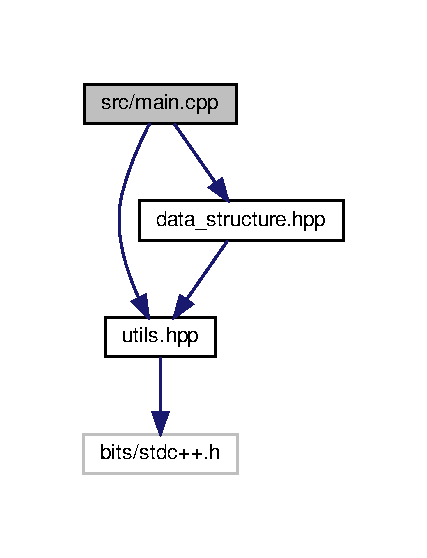
\includegraphics[width=205pt]{main_8cpp__incl}
\end{center}
\end{figure}
\subsection*{Functions}
\begin{DoxyCompactItemize}
\item 
\mbox{\Hypertarget{main_8cpp_ae66f6b31b5ad750f1fe042a706a4e3d4}\label{main_8cpp_ae66f6b31b5ad750f1fe042a706a4e3d4}} 
int {\bfseries main} ()
\end{DoxyCompactItemize}

\hypertarget{utils_8hpp}{}\section{src/utils.hpp File Reference}
\label{utils_8hpp}\index{src/utils.\+hpp@{src/utils.\+hpp}}
{\ttfamily \#include $<$bits/stdc++.\+h$>$}\newline
Include dependency graph for utils.\+hpp\+:\nopagebreak
\begin{figure}[H]
\begin{center}
\leavevmode
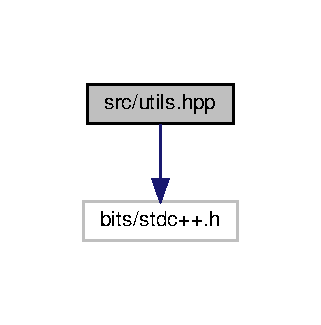
\includegraphics[width=154pt]{utils_8hpp__incl}
\end{center}
\end{figure}
This graph shows which files directly or indirectly include this file\+:\nopagebreak
\begin{figure}[H]
\begin{center}
\leavevmode
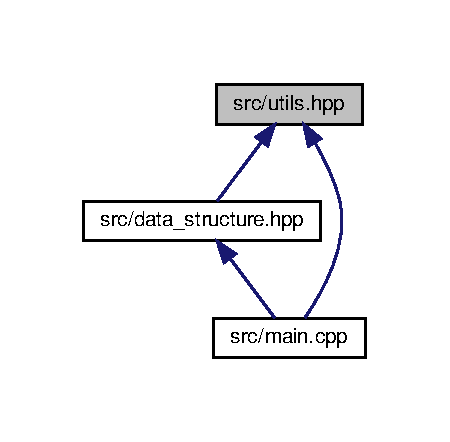
\includegraphics[width=216pt]{utils_8hpp__dep__incl}
\end{center}
\end{figure}
\subsection*{Macros}
\begin{DoxyCompactItemize}
\item 
\mbox{\Hypertarget{utils_8hpp_a8091c2bcff55cbe0a4a145fd5fb7c22d}\label{utils_8hpp_a8091c2bcff55cbe0a4a145fd5fb7c22d}} 
\#define {\bfseries F\+A\+ST}~ios\+\_\+base\+::sync\+\_\+with\+\_\+stdio(0),cin.\+tie(0),cout.\+tie(0)
\item 
\mbox{\Hypertarget{utils_8hpp_a795dcd1c94d9a983e5f1a7485a8efddf}\label{utils_8hpp_a795dcd1c94d9a983e5f1a7485a8efddf}} 
\#define {\bfseries dofloat}~cout$<$$<$fixed$<$$<$setprecision(8)
\item 
\mbox{\Hypertarget{utils_8hpp_a276c5a0e984cf60015b27252fe04fe6b}\label{utils_8hpp_a276c5a0e984cf60015b27252fe04fe6b}} 
\#define {\bfseries pb}~push\+\_\+back
\item 
\mbox{\Hypertarget{utils_8hpp_aea466a7139309b17bce61d5ccb03e195}\label{utils_8hpp_aea466a7139309b17bce61d5ccb03e195}} 
\#define {\bfseries mp}~make\+\_\+pair
\item 
\mbox{\Hypertarget{utils_8hpp_ad4fc2abd8f65bfb50ef452d359f38802}\label{utils_8hpp_ad4fc2abd8f65bfb50ef452d359f38802}} 
\#define {\bfseries fi}~first
\item 
\mbox{\Hypertarget{utils_8hpp_a3a9d1c7e37d1ab10d1044a1e43860aef}\label{utils_8hpp_a3a9d1c7e37d1ab10d1044a1e43860aef}} 
\#define {\bfseries se}~second
\item 
\mbox{\Hypertarget{utils_8hpp_a1d9b2b6e98a6f105a6482ffb91709a0c}\label{utils_8hpp_a1d9b2b6e98a6f105a6482ffb91709a0c}} 
\#define {\bfseries bitcount}~\+\_\+\+\_\+builtin\+\_\+popcount
\item 
\mbox{\Hypertarget{utils_8hpp_a9e11a37314dba5da17749442c5a200bf}\label{utils_8hpp_a9e11a37314dba5da17749442c5a200bf}} 
\#define {\bfseries all}(vec)~vec.\+begin(),vec.\+end()
\item 
\mbox{\Hypertarget{utils_8hpp_ae7bbf43e0ac300ac44df08d3aca48142}\label{utils_8hpp_ae7bbf43e0ac300ac44df08d3aca48142}} 
\#define {\bfseries rall}(vec)~vec.\+rbegin(),vec.\+rend()
\end{DoxyCompactItemize}
\subsection*{Typedefs}
\begin{DoxyCompactItemize}
\item 
\mbox{\Hypertarget{utils_8hpp_a649842e78f219114435121a088c1bed2}\label{utils_8hpp_a649842e78f219114435121a088c1bed2}} 
typedef long long {\bfseries ll}
\item 
\mbox{\Hypertarget{utils_8hpp_a09bfe86a130ac3370740e01ab26b8b48}\label{utils_8hpp_a09bfe86a130ac3370740e01ab26b8b48}} 
typedef long double {\bfseries ld}
\item 
\mbox{\Hypertarget{utils_8hpp_a1698594ea655b7b6fe3abe8a22556446}\label{utils_8hpp_a1698594ea655b7b6fe3abe8a22556446}} 
typedef vector$<$ long long $>$ {\bfseries vl}
\item 
\mbox{\Hypertarget{utils_8hpp_a2d381df6efdce67d2af04bbb25013ef2}\label{utils_8hpp_a2d381df6efdce67d2af04bbb25013ef2}} 
typedef pair$<$ long long, long long $>$ {\bfseries pll}
\item 
\mbox{\Hypertarget{utils_8hpp_a1acf30fb46927c25b8cec2b55cd10643}\label{utils_8hpp_a1acf30fb46927c25b8cec2b55cd10643}} 
typedef vector$<$ pair$<$ long long, long long $>$ $>$ {\bfseries vll}
\item 
\mbox{\Hypertarget{utils_8hpp_a865b1f6578b54b38c1b9e662ca451c8c}\label{utils_8hpp_a865b1f6578b54b38c1b9e662ca451c8c}} 
typedef vector$<$ pair$<$ int, int $>$ $>$ {\bfseries vii}
\item 
\mbox{\Hypertarget{utils_8hpp_a2954e26aee7d16c4a58d5cfb5571ea7e}\label{utils_8hpp_a2954e26aee7d16c4a58d5cfb5571ea7e}} 
typedef vector$<$ int $>$ {\bfseries vi}
\item 
\mbox{\Hypertarget{utils_8hpp_a08126f4b53dd101dbde6e02c82580cf0}\label{utils_8hpp_a08126f4b53dd101dbde6e02c82580cf0}} 
typedef pair$<$ int, int $>$ {\bfseries ii}
\end{DoxyCompactItemize}
\subsection*{Variables}
\begin{DoxyCompactItemize}
\item 
\mbox{\Hypertarget{utils_8hpp_af00b30d9f762b264076ba57ecc221c91}\label{utils_8hpp_af00b30d9f762b264076ba57ecc221c91}} 
const long long {\bfseries M\+OD} =1000000007
\item 
\mbox{\Hypertarget{utils_8hpp_a96e1c8d1ca0088289b1dcf367deb8018}\label{utils_8hpp_a96e1c8d1ca0088289b1dcf367deb8018}} 
const long long {\bfseries M\+AX} =100005
\item 
\mbox{\Hypertarget{utils_8hpp_acf20630e5d2a9696928fe77b0726013c}\label{utils_8hpp_acf20630e5d2a9696928fe77b0726013c}} 
const long double {\bfseries PI} =3.\+14159265359
\item 
\mbox{\Hypertarget{utils_8hpp_a977abf14dc0cd94cbd397c08d5ffc1c8}\label{utils_8hpp_a977abf14dc0cd94cbd397c08d5ffc1c8}} 
const long double {\bfseries G} =9.\+807
\item 
\mbox{\Hypertarget{utils_8hpp_a762f303452b602b3c490cae71a8fa4aa}\label{utils_8hpp_a762f303452b602b3c490cae71a8fa4aa}} 
const long long {\bfseries I\+NF} =1e18
\item 
\mbox{\Hypertarget{utils_8hpp_a177918db7d15eee629917d44ab88f78b}\label{utils_8hpp_a177918db7d15eee629917d44ab88f78b}} 
const long double {\bfseries E\+PS} =1e-\/6
\end{DoxyCompactItemize}

%--- End generated contents ---

% Index
\backmatter
\newpage
\phantomsection
\clearemptydoublepage
\addcontentsline{toc}{chapter}{Index}
\printindex

\end{document}
